\scanpage{45}\mspage{44}
\uline{Corollary} If $\deleted{\unsure{X}}Y\ll X$, then \deleted{the relation} every open shadow of a \deleted{\unsure{figure|stratum of}} \inserted{effective stratum} $Y$ is contained in the open shadow of a stratum of $X$. More generally and consequently, for every figure $F$ and \deleted{\unsure{t}} \deleted{subfigure} \inserted{refinement} $F'$ of $F$, every \deleted{stratum} \deleted{of open shadow of a} open stratum of $F'$ is contained in a (unique) open stratum of $F$.

\deleted{\uline{\unsure{Cont|Cond}}. 8 If \unsure{/}}\enspace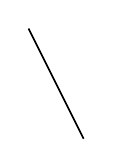
\begin{tikzpicture}[baseline=0pt]\draw[line width=.6pt] (0,.4)--(.7,-1);\end{tikzpicture}

I have just noticed that in the case of the pseudo disk, \deleted{a} two disjoint loci \deleted{\unsure{cq}} \inserted{$x,y$} of the interior (which therefore define two ``refinements'' of the said pseudo-disk), that there exists a ``Subdivision'' of the disk of which they are \unsure{nodes|nodes}. [\uline{NB}. The \uline{nodes} of a figure \inserted{$\deleted{F}F$} are the multistrata \inserted{of $\deleted{\unsure{X|F}}F$} reduced to a locus, i.e. the elements of $F\cap\mathcal L$] Thus \deleted{\unsure{the no}} there is no reason to consider $\{x,y\}$ as a ``refinement'', since it does not extend to a subdivision. Thus it is inappropriate
